\documentclass[10pt]{scrartcl}
% \documentclass[10pt]{article}
\usepackage[T1]{fontenc}
\usepackage{amsmath,amsfonts,amssymb}
\usepackage{mathtools}
\usepackage{color,soul}
\usepackage{fullpage}
\usepackage{enumerate}
\usepackage{graphicx}
\usepackage[colorlinks=true,urlcolor=blue]{hyperref}
\usepackage{floatrow}
\usepackage{deluxetable}
\usepackage{verbatim}
\usepackage{fancyvrb}
\usepackage{listings}
\usepackage{calc}
\usepackage[font=small]{caption}
\usepackage[font=scriptsize]{subcaption}

\floatsetup{ 
  heightadjust=object,
  valign=t
}

\definecolor{Light}{gray}{.90}
\sethlcolor{Light}

\title{Fitted Lines to Bundles}
\author{Jeren Suzuki}
\date{Last Edited \today}

\begin{document}

\maketitle
\pagenumbering{Roman}
\tableofcontents
\clearpage
\pagenumbering{arabic}

\section{Introduction} % (fold)
\label{sec:introduction}
With pictures taken with my camera, then fitted lines to edges of slats.
% section introduction (end)

\section{Starting Image} % (fold)
\label{sec:starting_image}

\begin{figure}[!ht]
    \centering
    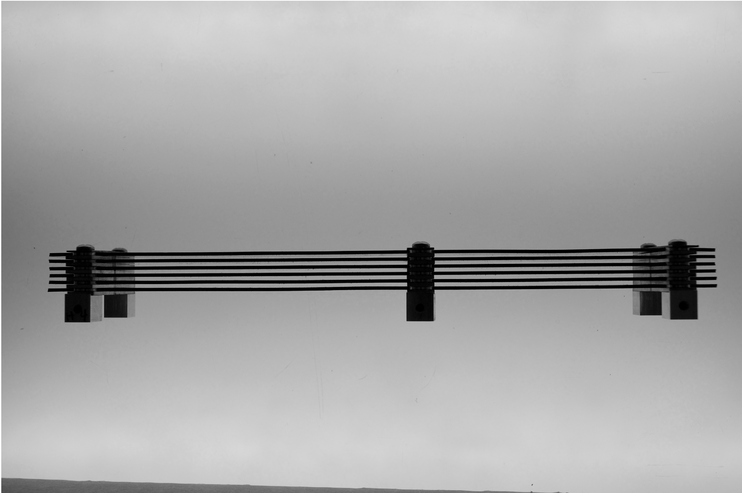
\includegraphics[width=.7\textwidth]{../plots_tables_images/wholebundle.png}
    \caption{Starting Image, red channel}
\end{figure}

Before we threshold the image to isolate the darkened slats, we have to de-noise the image. There is an option to de-noise the image in third-party post-processing software but it \emph{should} be done in IDL for the sake of completeness and control over data manipulation. FFT filtering is used, but it takes a long time. An option is to crop a region out of just the slats so that the analysis can be done quicker. 

\begin{figure}[!ht]
\ffigbox{
    \begin{subfloatrow}
        \ffigbox[1.5\FBwidth]% Width of subfloat
        {
        
\includegraphics[width=\linewidth]{../plots_tables_images/anofilt.eps}
        }
        {
        \subcaption{No filtering}
        }
    \end{subfloatrow} \\   
    \begin{subfloatrow}
        \ffigbox[.9\FBwidth]% Width of subfloat
        {
        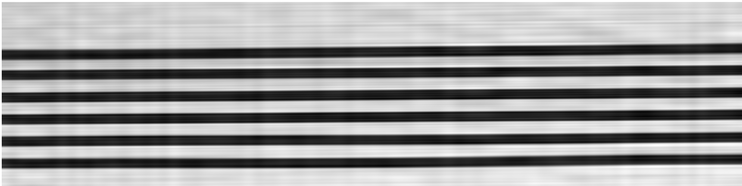
\includegraphics[width=\linewidth]{../plots_tables_images/wholefft.png}
        }
        {
        \subcaption{FFT'd on whole image, then cropped}
        }
    \end{subfloatrow}
    \begin{subfloatrow}
        \ffigbox[.9\FBwidth]% Width of subfloat
        {
        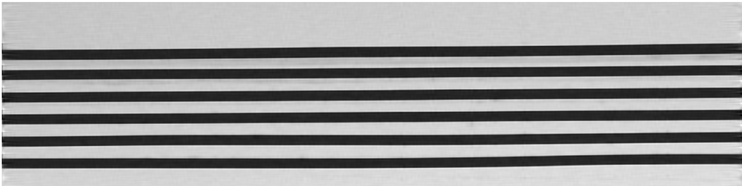
\includegraphics[width=\linewidth]{../plots_tables_images/cropfft.png}
        }
        {
        \subcaption{Cropped, then FFT'd}
        \label{pickme}
        }
    \end{subfloatrow}
}
{\caption{FFT Test}
\label{ffttest}}
\end{figure}

As you can see, using the FFT operator on the whole image resulted in some ringing and artifacts in the cropped region. 

% section starting_image (end)

\section{Fitted Lines} % (fold)
\label{sec:fitted_lines}

With a filtered image, I set a threshold to find the edges of the slats. The process is scalable to any number of slats. In Figure \ref{badfit}, a particularly curved edge of a slat results in a weird shape but upon closer inspection, the variance from the edges of the slat only differs by 10 pixels. With all slats edge-fitted, a color check on the processed image is performed, as in Figure \ref{test}.

\begin{figure}[!ht]
\ffigbox{
    \begin{subfloatrow}
        \ffigbox[.9\FBwidth]% Width of subfloat
        {
        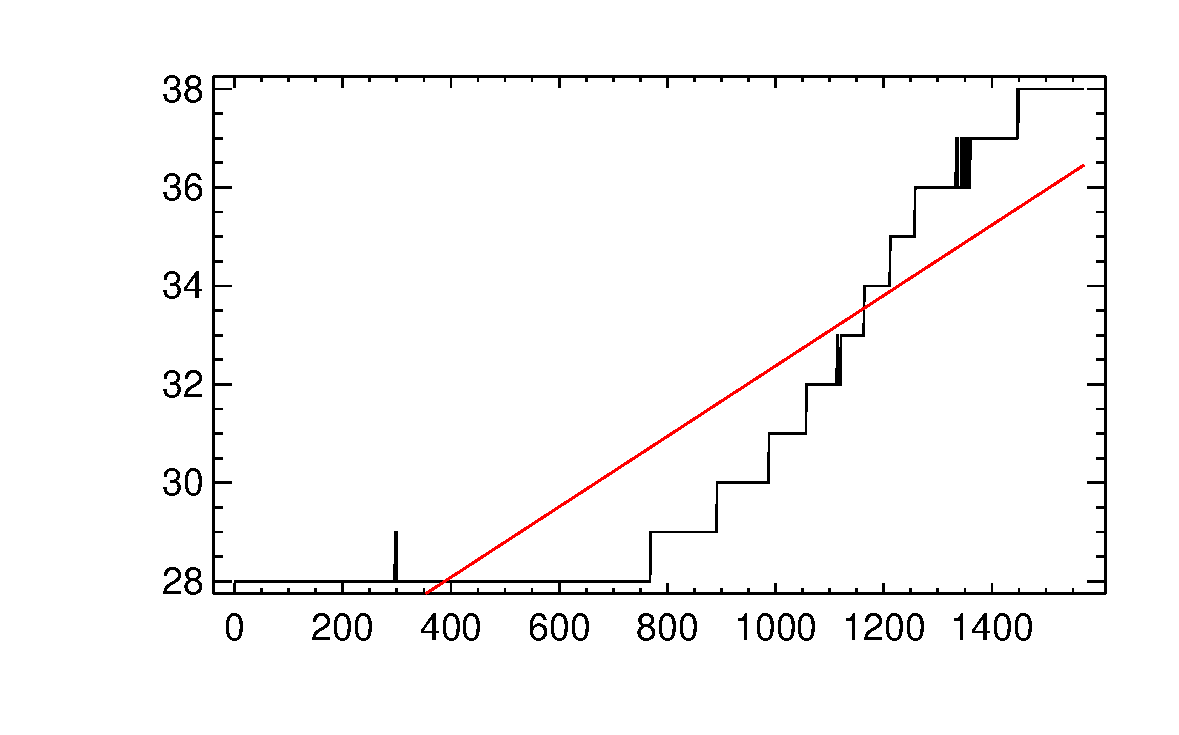
\includegraphics[width=\linewidth]{../plots_tables_images/edgefit0}
        }
        {
        \subcaption{Linear fitting the edge of a slat}
        \label{badfit}
        }
    \end{subfloatrow}
    \begin{subfloatrow}
        \ffigbox[.9\FBwidth]% Width of subfloat
        {
        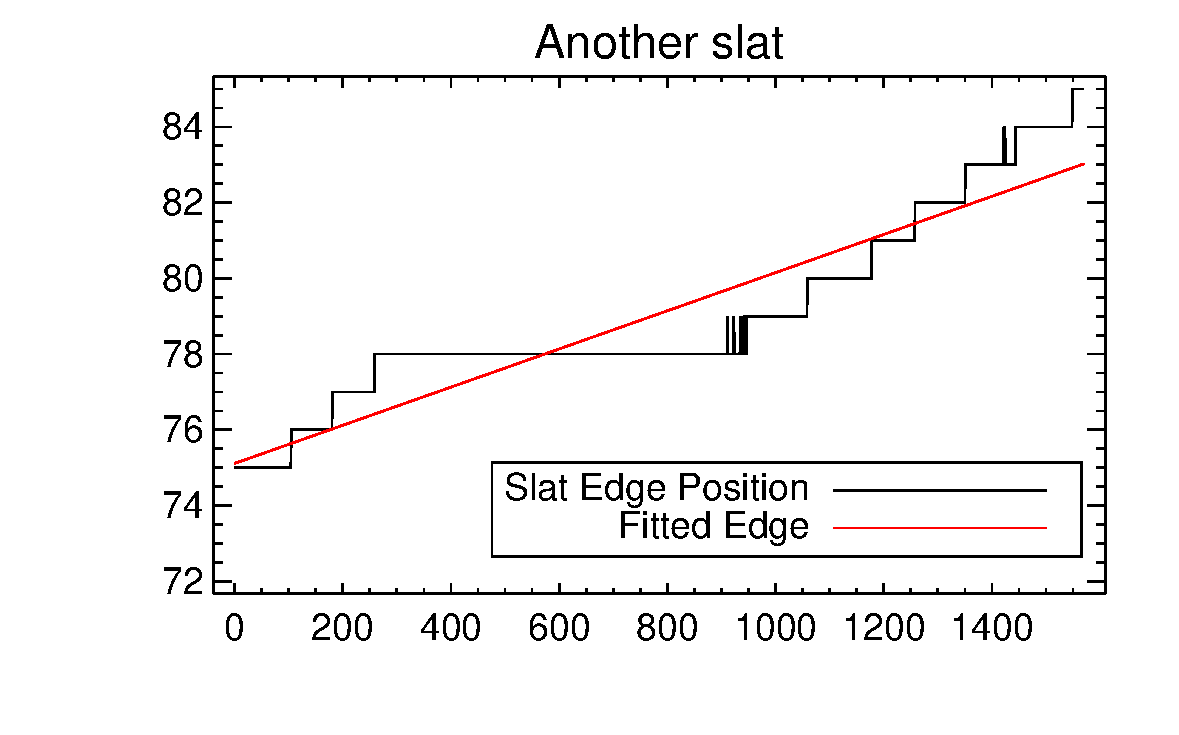
\includegraphics[width=\linewidth]{../plots_tables_images/edgefit1}
        }
        {
        \subcaption{Linear fitting the edge of another slat}
        }
    \end{subfloatrow}
}
{\caption{}
\label{edgefit}}
\end{figure}


\begin{figure}[!ht]
    \centering
    
\includegraphics[width=\textwidth]{../plots_tables_images/lines}
    \caption{Cropped region of slats with edges of slats marked in color}
    \label{test}
\end{figure}


% section fitted_lines (end)


\section{Bundle Analysis Steps} % (fold)
\label{sec:bundle_analysis_steps}

To start off with, I use FFT filtering to get rid of the dust and high spatial noise in our image. Once I get Figure \ref{pickme}, I take vertical slices and threshold the slats below a certain value. In Figure \ref{findedge}, the top plot illustrates the slat structure while the bottom plot is thresholded to values lower than 20.

\begin{figure}[!ht]
    \centering
    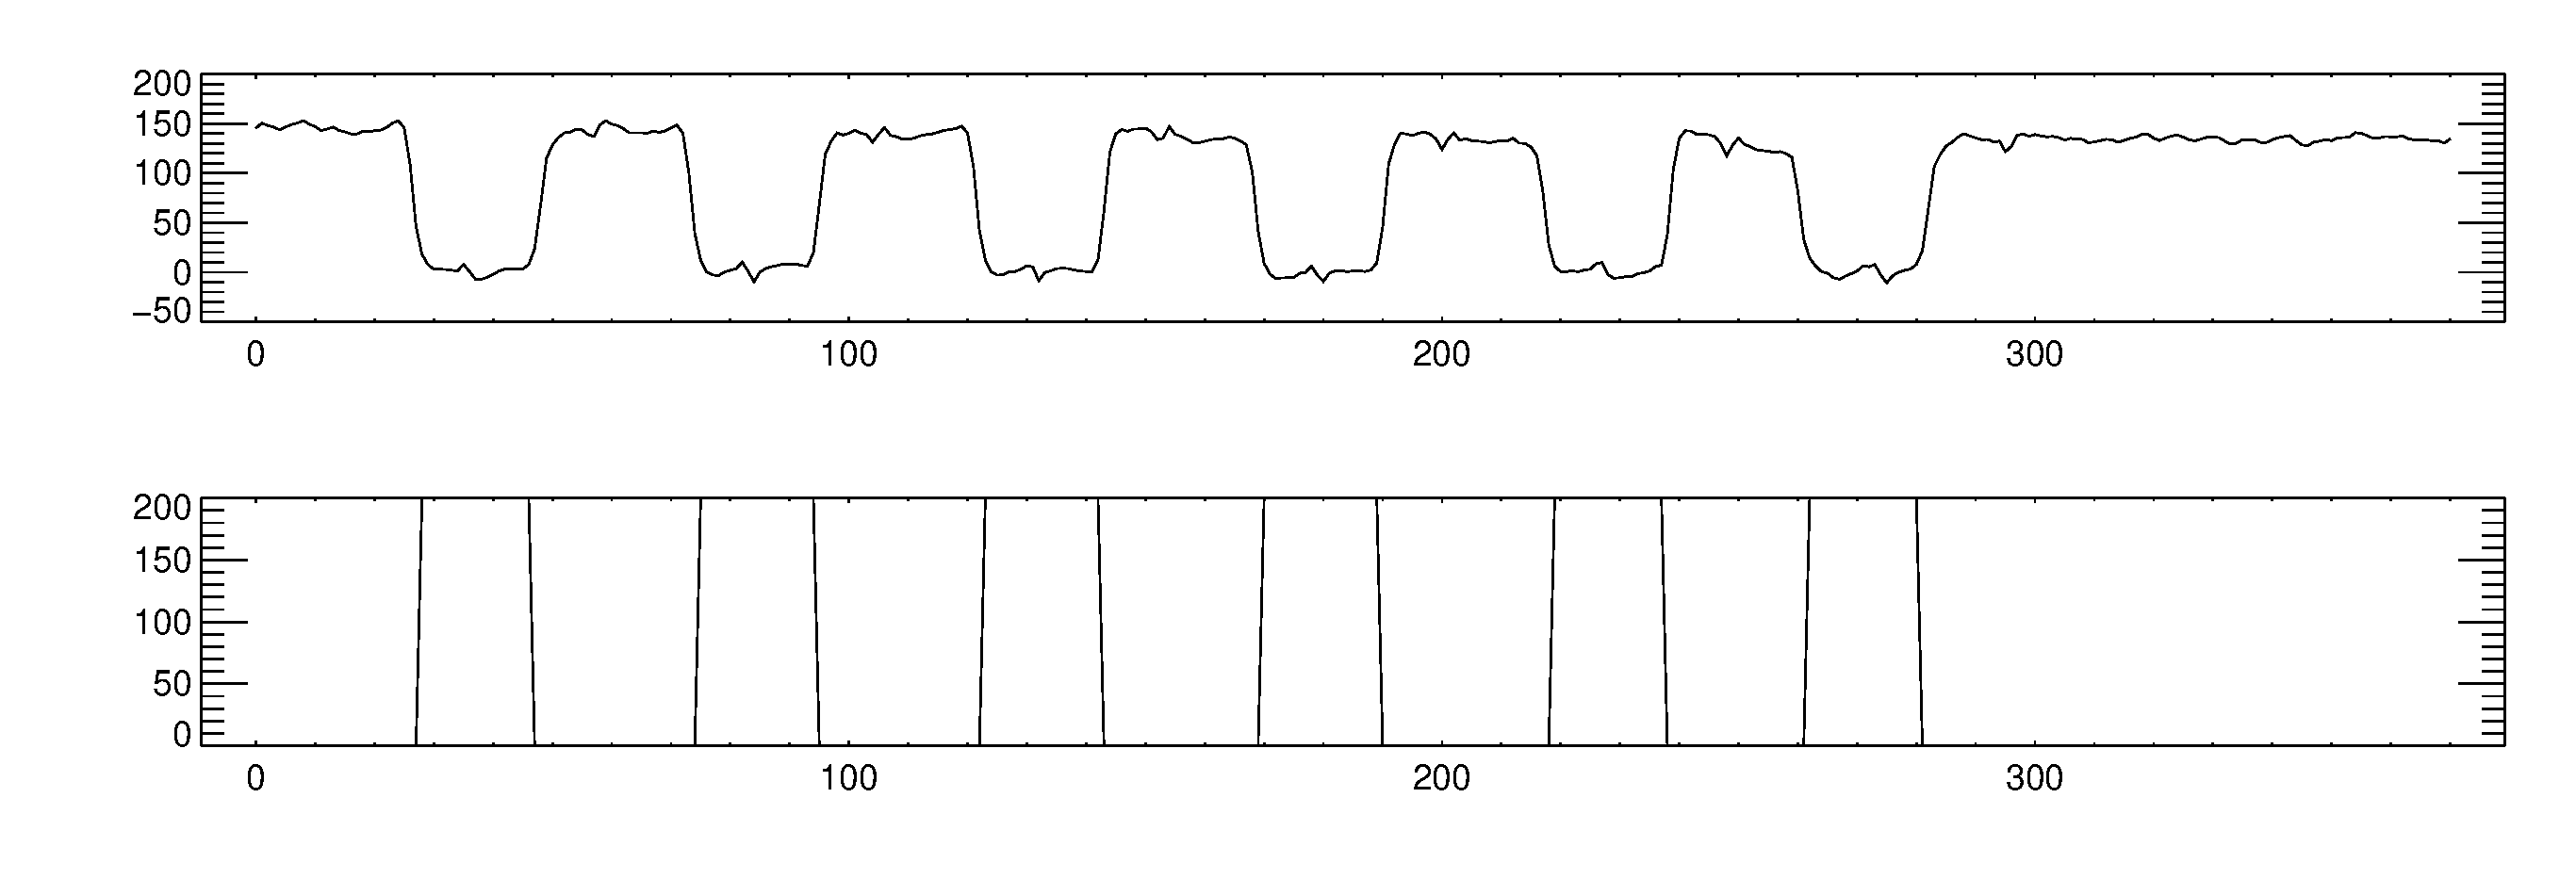
\includegraphics[width=.8\textwidth]{../plots_tables_images/findedge}
    \caption{}
    \label{findedge}
\end{figure}

With these edges, I find where values of \hl{\texttt{array - shift(array,1)}} equal 1 and where \hl{\texttt{array - shift(array,-1)}} equal -1, which correspond to the edges of each pillar structure. These positions are stuck into two 6xN length matrices, one for each edge of the slat. Now I move on to the next column, do a \hl{\texttt{shift()}} check and append the next 6 pairs into the 6xN arrays. Once finished, I fit each row of the 6xN array to a line and overplot the line position into the 2D starting image, as per Figure \ref{test}.

% section bundle_analysis_steps (end)




\end{document}